\section{Introduction}
\label{sec:introduction}

\par The main objective of this laboratory assignment is to implement a BandPass Filter (BPF) with a central frequency of 1kHz and a gain at the central frequency of 40dB, reaching the best figure of merit possible. In order to this, the architecture of the circuit had to be chosen following a few restrictions in terms of the components that were allowed to use. The merit of the circuit is given by:

\begin{equation}
  M = \frac {1}{cost * (voltage gain deviation + central frequency deviation + 10^-6)}.
  \label{eq:merit}
\end{equation}


\par The circuit used to produce the BandPass Filter is shown in Figure\ref{fig:circuit}.

\begin{figure}[h] \centering
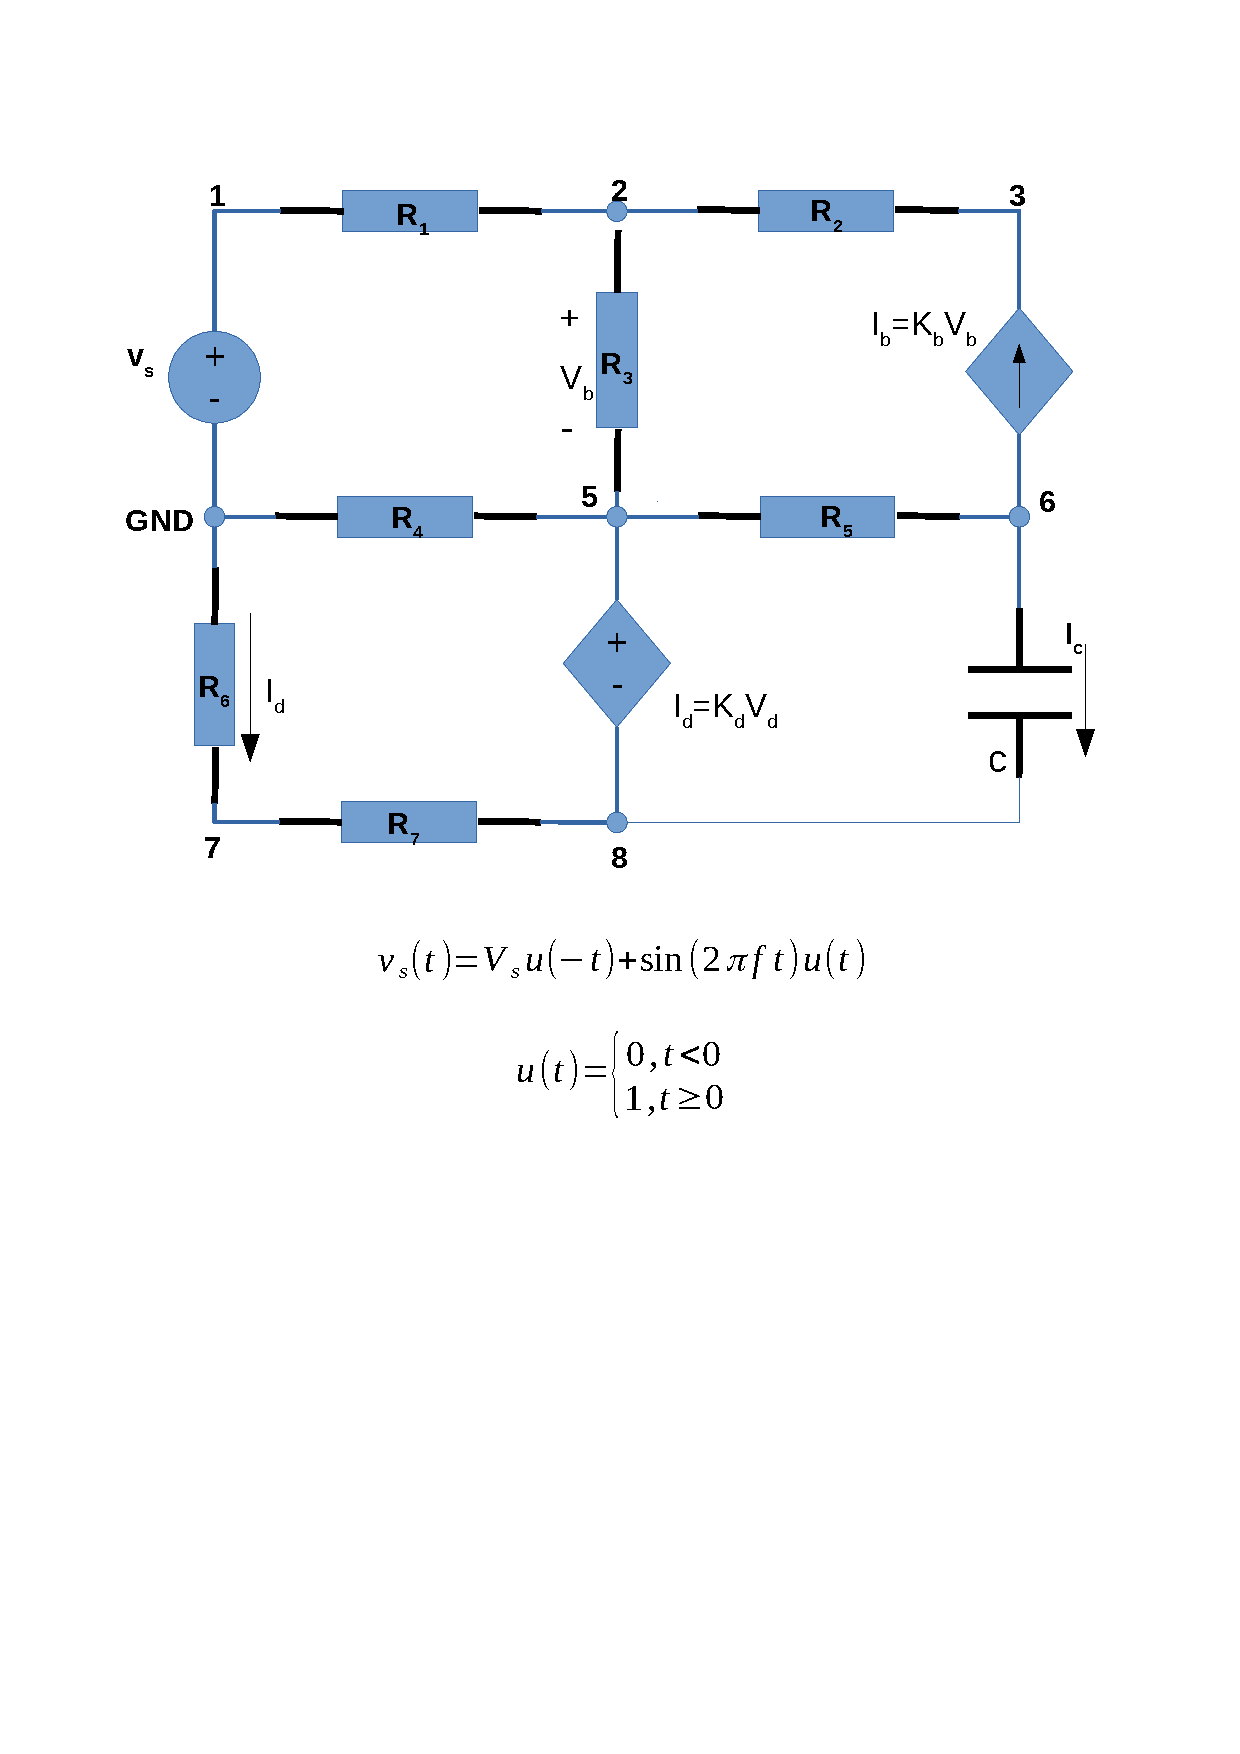
\includegraphics[width=0.6\linewidth]{circuit.pdf}
\caption{Circuit under analysis.}
\label{fig:circuit}
\end{figure}


\par In the next section (~\ref{sec:analysis}), we briefly explain the procedure to analyse theoretically the circuit above with the use of Octave maths tool. In Section 3 a simulation analysis is given, where we resorted to Ngspice to simulate the circuit, and a few graphics are presented to understand the results. The report finishes with its conclusion in section~\ref{sec:conclusion}, where we analyse side by side the theoretical and simulated results and resume the most important points of the lab assignment.

\newpage
